\documentclass{report}
\usepackage[margin=1in, paperwidth=8.5in, paperheight=11in]{geometry}
%Math packages%
\usepackage{amsmath}
\usepackage{amsthm}
%Spacing%
\usepackage{setspace}
\onehalfspacing
%Lecture number%
\newcommand{\lectureNum}{5}
%Variables - Date and Course%
\newcommand{\curDate}{January 17, 2017}
\newcommand{\course}{CS 240}
%Defining the example tag%
%\theoremstyle{definition}%
\newtheorem{ex}{Example}[section]
%Setting counter given the lecture number%
\setcounter{chapter}{\lectureNum{}}
%Package to insert code%
\usepackage{listings}
\usepackage{courier}
\usepackage{xcolor}
\lstset { 
    tabsize=2,
    breaklines=true,
    language=C++,
    backgroundcolor=\color{blue!8}, % set backgroundcolor
    basicstyle=\footnotesize\ttfamily,% basic font setting
}
%Package to draw trees%
\usepackage{tikz}

\begin{document}
%Note title%
\begin{center}
\begin{Large}
\textsc{\course{} | Lecture \lectureNum{}}
\end{Large}
\end{center} 
\noindent \textit{Bartosz Antczak} \hfill
\textit{Instructor: Eric Schost} \hfill
\textit{\curDate{}}
\rule{\textwidth}{0.4pt}

% Actual Notes%
\section{The Height of a Heap}
\begin{ex}
Consider the following heap:
\end{ex}
%HEAP 1%
\begin{center}
\begin{tikzpicture}[
  level distance=40 pt,
  every node/.style={circle,draw},
  level 1/.style={sibling distance=200 pt},
  level 2/.style={sibling distance=100 pt},
  level 3/.style={sibling distance=60 pt}
]
  \node {20}
    child {node {10}
      child {node {9}
      	child {node {6}}
      	child {node {6}}}
      child {node {7}
      	child {node {3}}
      	child [missing]}
    }
    child {node {19}
      child {node {2}}
      child {node {1}}
    };
\end{tikzpicture}
\end{center}
We observe that the height of the heap is 3, and there are 10 nodes. There is/are:
\begin{itemize}
\item 1 node at level 0
\item 2 nodes at level 1
\item 4 nodes at level 2
\end{itemize}
We also observe that there are between 1 and 8 nodes at level 3. This means that for a heap of height $h=3$, the number $n$ of nodes satisfies
$$1+2+4+1 \leq n \leq 1+2+4+8$$
(i.e., the least number of nodes this heap can have is $1+2+4+1$, and th max number it can have is $1+2+4+8$).\\
In general, we have
\begin{align}
1+2+4+\cdots+2^{h-1} + 1 \leq \, &n \leq 1+2+4+\cdots + 2^{h-1} + 2^h \\
2^h \leq \, &n \leq 2^{h+1} -1 \leq 2^{h+1} \\
h \leq & \, \log_2(n) \leq h+1 \\
\log_2(n)-1 \leq \, &h \leq \log_2(n)
\end{align}
On line 5.2, we used the identity $\displaystyle \sum_{i=1}^n 2^i = 2^{n+1} - 1$. From line 5.4, we see that the time it takes to traverse the height of a heap with $n$ nodes is $\in \Theta(\log_2 n)$.
\section{Building Heaps Using Arrays}
To work with heaps in code, we store it in an array. Consider a heap $H$ of $n$ items. We'll create an array $A$ of size $n$. We store the root in $A[0]$, and we continue with the elements level-by-level from top to bottom, in each level left to right. To access
\begin{itemize}
\item the left child of $A[i]$, go to $A[2i + 1]$
\item the right child of $A[i]$, go to $A[2i + 2]$
\item the parent of $A[i]$ ($i \neq 0$), go to $A[\lfloor\frac{i-1}{2}\rfloor]$
\end{itemize}
The array implementation of the heap from example 5.1.1 would be $A = [20, 10, 5, 9, 7, 2, 1, 6, 6, 3]$.
\subsection{Various Algorithms to Implement Heaps}
\textbf{Problem:} Given $n$ items in $A[0 \cdots n-1]$, build a heap containing all of them.
\subsubsection{Approach 1}
This approach starts with an empty heap and inserts nodes one at a time. Analysing this algorithm, we see that the worst case running time will involve \textit{bubbling-up} on every insertion. This means that inserting the $i$th element may take $\log_2 (i)$ swaps (recall that this defines the time it takes to traverse the height of a heap), which means that the worst case running time is
\begin{align*}
&\Theta\left(\sum_{i=1}^n \log_2 (i)\right) \\
&\Theta(\log_2 (n!)) \\
&\Theta(n \log_2 n)
\end{align*}
\subsubsection{Approach 2}
Remember that we're working with heaps structured as arrays. So instead of manually inserting one node at a time, it would seem faster to simply take an arbitrary array, and apply the \textit{bubble-down} algorithm on the first $\frac{n}{2}$ nodes, starting with the node at index $\lfloor \frac{n}{2} \rfloor$, going down to the root node (index 0). Applying this bubble-down implementation grantees that this array will be a proper heap.
\begin{ex}
Applying this algorithm on an arbitrary array (in heap form):
\end{ex}
%Four heaps, showing the step process%
%Heap 1%
\begin{center}
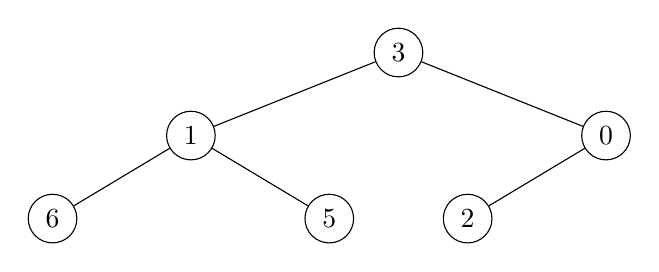
\begin{tikzpicture}[
  level distance=30 pt,
  every node/.style={circle,draw},
  level 1/.style={sibling distance=150 pt},
  level 2/.style={sibling distance=100 pt},
  level 3/.style={sibling distance=60 pt}
]
  \node {3}
    child {node {1}
      child {node {6}}
      child {node {5}}
    }
    child {node {0}
      child {node {2}}
      child [missing]
    };
\end{tikzpicture}
\\ \textbf{1.} We start with an arbitrary heap. \\
\end{center}
%Heap 2%
\begin{center}
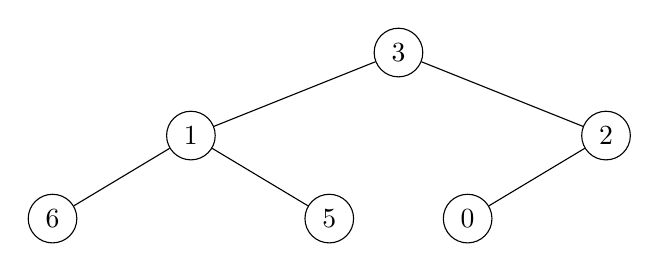
\begin{tikzpicture}[
  level distance=30 pt,
  every node/.style={circle,draw},
  level 1/.style={sibling distance=150 pt},
  level 2/.style={sibling distance=100 pt},
  level 3/.style={sibling distance=60 pt}
]
  \node {3}
    child {node {1}
      child {node {6}}
      child {node {5}}
    }
    child {node {2}
      child {node {0}}
      child [missing]
    };
\end{tikzpicture}
\\ \textbf{2.} Bubble down on index index two (which is $\lfloor \frac{n}{2}\rfloor$ | node ``0") \\
\end{center}
%Heap 3%
\begin{center}
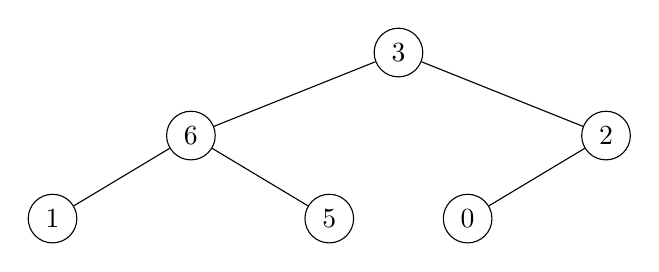
\begin{tikzpicture}[
  level distance=30 pt,
  every node/.style={circle,draw},
  level 1/.style={sibling distance=150 pt},
  level 2/.style={sibling distance=100 pt},
  level 3/.style={sibling distance=60 pt}
]
  \node {3}
    child {node {6}
      child {node {1}}
      child {node {5}}
    }
    child {node {2}
      child {node {0}}
      child [missing]
    };
\end{tikzpicture}
\\ \textbf{3.} Bubble down on index one | node ``1" \\
\end{center}
%Heap 2%
\begin{center}
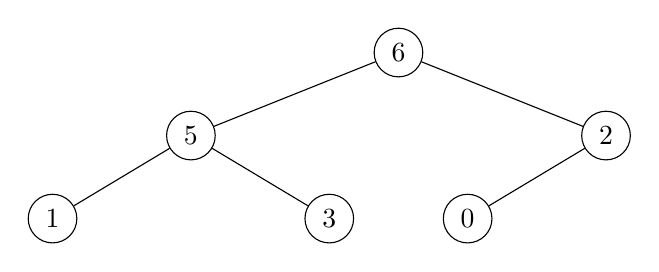
\begin{tikzpicture}[
  level distance=30 pt,
  every node/.style={circle,draw},
  level 1/.style={sibling distance=150 pt},
  level 2/.style={sibling distance=100 pt},
  level 3/.style={sibling distance=60 pt}
]
  \node {6}
    child {node {5}
      child {node {1}}
      child {node {3}}
    }
    child {node {2}
      child {node {0}}
      child [missing]
    };
\end{tikzpicture}
\\ \textbf{4.} Finally, bubble-down on index zero | node ``3" \\
\end{center}
Analyzing this algorithm on a tree of height 3, we see that in the worst case running time
\begin{itemize}
\item On level $h=3$, we perform 0 swaps (since all nodes are leaves in this level)
\item On level $h-1 = 2$, we perform $4 \times 1$ swaps
\item On level $h-2 = 1$, we perform $2 \times 2$ swaps
\item On level $h-3 = 0$, we perform $h=3$ swaps
\end{itemize}
In general, the number of swaps is at most
$$(1 \cdot h) + (2 \cdot (h-1)) + (4 \cdot (h-2)) + \cdots + (2^{h-1} \cdot 1)$$
which can be simplified to
\begin{align*}
&= (2^0 \cdot (h-0)) + (2^1 \cdot (h-1)) + (2^2 \cdot (h-2)) + \cdots + (2^{h-1} \cdot (h - (h-1))) \\
&= \sum_{i=0}^{h-1} 2^i \cdot (h-i) \\
&= 2^h \sum_{i=0}^{h-1} 2^{i-h} \cdot (h-i) \\
&= 2^h \sum_{i=0}^{h-1} \frac{h-i}{2^{h-i}}\\
&\leq 2 \leq 2 \cdot 2^h \leq 2n && \text{(From equation 5.4)}
\end{align*}
Thus, the runtime of this algorithm is $\in \Theta(n)$.
\section{Intro to Selection}
The \textbf{selection problem} states:
\begin{center}
\textit{Given an array $A$ of $n$ numbers, and $0 \leq k \leq n$, find the element in position $k$ of the sorted array (a.k.a. the $k$-th largest number in $A$)}
\end{center}
Consider input array $A = [3,2,8,7,6,11,12,22,1]$
\subsection{Quick-select and Quick-sort}
These two algorithms are used to sort an array. They rely on two important subroutines (in linear time):
\begin{itemize}
\item choose-pivot
\item partition
\end{itemize}
More on this in the next lecture
%END%
\end{document}